\documentclass{article}
\usepackage[a4paper, tmargin=1in, bmargin=1in]{geometry}
\usepackage[utf8]{inputenc}
\usepackage{graphicx}
\usepackage[justification=centering]{caption}

% \usepackage{parskip}
\usepackage{pdflscape}
\usepackage{listings}
\usepackage{hyperref}
\usepackage{caption}
\usepackage{subcaption}
\usepackage{float}
\usepackage{enumerate}
\usepackage{amsmath}

\setlength{\parindent}{0pt}

\title{CS 754 : Advanced Image ProcessingAssignment 2}
\author{Meet Udeshi - 14D070007\\
  Arka Sadhu - 140070011\\
}
\date{\today}

\newcommand{\lone}[1]{
  ||#1||_{l_1}
}
\newcommand{\ltwo}[1]{
  ||#1||_{l_2}
}
\newcommand{\linf}[1]{
  ||#1||_{l_\infty}
}
\newcommand{\htj}[1]{
  h_{T_{#1}}
}

\newcommand{\htc}[1]{
  h_{{#1}^c}
}

\newcommand{\hto}[1]{
  h_{#1}
}
\newcommand{\htzo}{
  h_{(T_0 \cup T_1)}
}

\newcommand{\htzoc}{
  h_{(T_0 \cup T_1)^c}
}

\begin{document}
\maketitle
\section*{Q1}
\subsection*{A1.1}
Need to show :
\begin{equation}\label{eq:1}
  \ltwo{h_{T_j}} \le s^{1/2} \linf{h_{T_j}}
\end{equation}
Equivalently we need to show :
$$\ltwo{A} \le s^{1/2} \linf{A}$$
where $A$ is a s-sparse vector.
Therefore
$$\ltwo{A} = \sqrt{\sum_{i}a_i^2} \le \sqrt{\sum_i max(a_i)^2} \le s^{1/2}max(a_i) = \linf{A}$$
The $s^{1/2}$ term comes from the fact that A is s-sparse matrix, and hence there will be at most s non-zero elements.

\subsection*{A1.2}
Need to show :
\begin{equation}\label{eq:2}
  s^{1/2}\linf{h_{T_j}} \le s^{-1/2}\lone{\htj{j-1}}
\end{equation}

for all $j \ge 2$\\\\
Equivalently we need to show :
$$s\linf{\htj{j}} \le \lone{\htj{j-1}}$$
From the definition of $T_j$ it follows for $j \ge 2$ that all elements of $\htj{j}$ will be less than the smallest non-zero element of
$\htj{j-1}$. Also both $\htj{j}$ and $\htj{j-1}$ are s-sparse matrix, hence it clearly follows that
$$s \linf{\htj{j}} = s*max(\htj{j}) \le \sum_i |\htj{j-1}| = \lone{\htj{j-1}} $$

\subsection*{A1.3}
Need to show :
\begin{equation}\label{eq:3}
  \sum_{j \ge 2} \ltwo{\htj{j}} \le s^{-1/2}(\lone{\htj{1}} + \lone{\htj{2}} + ...)
\end{equation}

This follows directly from \ref{eq:1} and \ref{eq:2}.
$$\ltwo{\htj{j}} \le s^{-1/2} \lone{\htj{j-1}}$$
for all $j \ge 2$
Now summing over all $j \ge 2$ we get
$$\sum_{j \ge 2} \ltwo{\htj{j}} \le s^{-1/2}(\lone{\htj{1}} + \lone{\htj{2}} + ...)$$

\subsection*{A1.4}
Need to show:
\begin{equation}
  \label{eq:4}
  s^{-1/2}(\lone{\htj{1}} + \lone{\htj{2}} + ...) \le s^{-1/2}\lone{\htc{T_0}}
\end{equation}
We note all of $\htj{1}$, $\htj{2}$ all have disjoint support and therefore
$$\lone{\htj{1}} + \lone{\htj{2}} + ... \le \lone{\htc{T_0}}$$



\subsection*{A1.5}
Need to show:
\begin{equation}
  \label{eq:5}
  \ltwo{\htc{(T_0 \cup T_1)}} = \ltwo{\sum_{j \ge 2}\htj{j}}
\end{equation}

We note that $$\htc{(T_0 \cup T_1)} = h - \hto{T_0} - \hto{T_1} = \hto{T_2} + \hto{T_3} + ... = \sum_{j \ge 2} \hto{T_j}$$

And hence \ref{eq:5} follows directly.

\subsection*{A1.6}
Need to show:
\begin{equation}
  \label{eq:6}
  \ltwo{\sum_{j \ge 2}{\htj{j}}} \le \sum_{j \ge 2} \ltwo{\htj{j}}
\end{equation}

This is simple extension of triangle inequality, which states that
$$|a+b| \le |a| + |b|$$
For n vectors it is simply
$$|a_1 + a_2 + a_3 +... +a_n| \le |a_1| + |a_2| + |a_3| + ... + |a_n| $$
And hence \ref{eq:6} follows directly

\subsection*{A1.7}
Need to show:
\begin{equation}
  \label{eq:7}
  \sum_{j \ge 2} \ltwo{\htj{j}} \le s^{-1/2}\lone{\htc{T_0}}
\end{equation}

This follows directly from \ref{eq:3} and \ref{eq:4}.
$$\sum_{j \ge 2} \ltwo{\htj{j}} \le s^{-1/2}(\lone{\htj{1}} + \lone{\htj{2}} + ...) \le s^{-1/2}\lone{\htc{T_0}}$$
\subsection*{A1.8}
Need to show:
\begin{equation}
  \label{eq:8}
  \lone{x} \ge \lone{x+h} \ge \lone{x_{T_0}} - \lone{\hto{T_0}} + \lone{\htc{T_0}} - \lone{x_{T_0^c}}
\end{equation}
For first part we note that $x^* = x + h$ therefore, $\lone{x^*} = \lone{x + h}$. According to our constraints,$x^*$ has the minimum $\lone{x^*}$ which also satisfies $\ltwo{y - \Phi x} \le \varepsilon$. Therefore if $x$ is not s-sparse then
$$\lone{x} > \lone{x^*}$$
And if $x$ is s-sparse then $$\lone{x} = \lone{x^*}$$
Combining the two we can say
$$\lone{x} \ge \lone{x^*}$$
From Triangle Inequality we know
$$\lone{a+b} \ge |\lone{a} - \lone{b}|$$
Therefore, we can also say
$$\lone{a+b} \ge \lone{a} - \lone{b}$$
And
$$\lone{a+b} \ge \lone{b} - \lone{a}$$
We note that
$$\lone{x+h} = \sum_{i \in T_0}|x_i + h_i| + \sum_{i \in T_0^c}|x_i + h_i| \ge \lone{x_{T_0}} - \lone{\hto{T_0}} + \lone{\htc{T_0}} - \lone{x_{T_0^c}}$$

\subsection*{A1.9}
Need to show:
\begin{equation}
  \label{eq:9}
  \ltwo{\htc{T_0}} \le \lone{\hto{T_0}} + 2\lone{x_{T_0^c}}
\end{equation}
We can rearrange \ref{eq:8} to have
$$\lone{\htc{T_0}} \le \lone{x} - \lone{x_{T_0}} + \lone{\hto{T_0}} + \lone{x_{T_0^c}}$$
We note that
$$\lone{x} - \lone{x_{T_0}} \le \lone{x - x_{T_0}} = \lone{x_{T_0^c}}$$
Therefore
$$\lone{\htc{T_0}} \le \lone{x_{T_0^c}} + \lone{\hto{T_0}} + \lone{x_{T_0^c}} = \lone{\hto{T_0}} + 2\lone{x_{T_0^c}}$$

\subsection*{A1.10}
Need to show:
\begin{equation}
  \label{eq:10}
  \ltwo{\htzoc} \le \ltwo{\hto{T_0}} + 2e_0, e_0 \equiv s^{-1/2}\ltwo{x - x_s}
\end{equation}

Combining \ref{eq:5} \ref{eq:6} and \ref{eq:7} we get
$$\ltwo{\htzoc} = \ltwo{\sum_{j \ge 2}\htj{j}} \le \sum_{j \ge 2} \ltwo{\htj{j}} \le s^{-1/2}\lone{\htc{T_0}}$$
From \ref{eq:9} we get
$$s^{-1/2}\lone{\htc{T_0}} \le s^{-1/2}\lone{\hto{T_0}} + 2s^{-1/2}\lone{x_{T_0^c}}$$
Also by definition
$$\lone{x_{T_0^c}} = \lone{x - x_s}$$
This implies
$$s^{-1/2}\lone{\htc{T_0}} \le s^{-1/2}\lone{\hto{T_0}} + 2s^{-1/2}\lone{x - x_s}$$
Therefore
$$s^{-1/2}\lone{\htc{T_0}} \le s^{-1/2}\lone{\hto{T_0}} + 2e_0, e_0 \equiv s^{-1/2}\ltwo{x - x_s}$$
Now we also note, for any s-sparse vector A
$$\lone{A} = \sum_i|a_i| = \sum_i |a_i|*1 \le \sqrt{s}\sqrt{\sum_i a_i^2} = s^{1/2}\ltwo{A}$$
and here we have used Cauchy Schwartz Inequality.
That is
$$s^{-1/2}\lone{A} \le \ltwo{A}$$
Thus it follows that 
$$s^{-1/2}\lone{\hto{T_0}} \le \ltwo{\hto{T_0}}$$
And \ref{eq:10} directly follows
$$\ltwo{\htzoc} \le \ltwo{\hto{T_0}} + 2e_0, e_0 \equiv s^{-1/2}\ltwo{x - x_s}$$

\subsection*{A1.14}
Need to show:
\begin{equation}
  \label{eq:14}
  \Phi \htzo = \Phi h - \sum_{j \ge 2}\Phi \htj{j}
\end{equation}
We know
$$\htzoc = h - \htzo =h - \hto{T_o} - \hto{T_1} = \sum_{j \ge 2}\htj{j}$$
Rearranging the equation
$$\htzo = h - \sum_{j \ge 2}\htj{j}$$
Multiplying $\phi$ on both sides
$$\Phi \htzo = \Phi h - \sum_{j \ge 2}\Phi \htj{j}$$

\subsection*{A1.15}
Need to show:
\begin{equation}
  \label{eq:15}
  |<\Phi\htzo,\Phi h>| \le \ltwo{\Phi\htzo}\ltwo{\Phi h}
\end{equation}

This is simple application of Cauchy Schwartz Inequality which states that given two vectors $a$ and $b$
$$<a,b> \le \ltwo{a}\ltwo{b}$$
And therefore \ref{eq:15} directly follows from this.

\subsection*{A1.16}
Need to show:
\begin{equation}
  \label{eq:16}
  \ltwo{\Phi\htzo}\ltwo{\Phi h} \le 2 \varepsilon \sqrt{1+\delta_{2s}}\ltwo{\htzo}
\end{equation}
We note that
$$\ltwo{\Phi(x^* - x)} \le \ltwo{\Phi x^* - y} + \ltwo{y - \Phi x} \le 2\varepsilon$$
The first part of the Inequality is a direct result of Traingle Inequality. The second part of the Inequality arises from the fact that
$\ltwo{y - \Phi x} \le \varepsilon$ and both $x$ and $x^*$ are a solution.
We have assumed $x^* = x + h$. Therefore
$$\ltwo{\Phi h} \le 2\varepsilon$$

Also from the definition of RIP
$$\sqrt{(1 - \delta_{s})} \ltwo{x} \le \ltwo{\Phi x} \le \sqrt{(1+\delta_s)} \ltwo{x}$$
where x is s-sparse vector.
We know that $\htzo$ is a 2s-sparse vector. Therefore
$$\ltwo{\Phi \htzo} \le \sqrt{(1+\delta_{2s})}\ltwo{\htzo}$$
Multiplying the inequalities directly gives \ref{eq:16}
$$\ltwo{\Phi\htzo}\ltwo{\Phi h} \le 2 \varepsilon \sqrt{1+\delta_{2s}}\ltwo{\htzo}$$

\subsection*{A1.17}
Need to show:
\begin{equation}
  \label{eq:17}
  \ltwo{\hto{T_0}} + \ltwo{\hto{T_1}} \le \sqrt{2}\ltwo{\htzo}
\end{equation}
From AM-GM Inequality we know
$$\ltwo{\hto{T_0}}\ltwo{\hto{T_1}} \le \frac{\ltwo{\hto{T_0}}^2 + \ltwo{\hto{T_1}}^2}{2}$$
Adding the RHS to both sides and Multiplying 2 on both sides
$$\ltwo{\hto{T_0} + \hto{T_1}}^2 \le 2\ltwo{\htzo}^2$$
Taking square roots on both sides gives us \ref{eq:17}

\subsection*{A1.18}
Need to show:
\begin{equation}
  \label{eq:18}
  (1-\delta_{2s})\ltwo{\htzo}^2 \le \ltwo{\Phi\htzo}^2
\end{equation}
Since $\htzo$ is a 2s-sparse vector, \ref{eq:18} follows from definition.

\subsection*{A1.19}
Need to show:
\begin{equation}
  \label{eq:19}
  \ltwo{\Phi\htzo}^2 \le \ltwo{\htzo} (2\varepsilon\sqrt{1+\delta_{2s}} + \sqrt{2}\delta_{2s}\sum_{j \ge 2}\ltwo{\htj{j}}) 
\end{equation}
Clearly
$$\ltwo{\Phi\htzo}^2 = <\Phi\htzo,\Phi h> - <\Phi \htzo, \sum_{j \ge 2}\htj{j}>$$
To get the maximum we want to maximize the first term and minimize the second term. As such we want to consider both
the absolute values. 
From \ref{eq:16}
$$\ltwo{\Phi\htzo}\ltwo{\Phi h} \le 2 \varepsilon \sqrt{1+\delta_{2s}}\ltwo{\htzo}$$
Also we note:
$$|<\Phi\htzo,\Phi\htj{j}>| \le |<\Phi\hto{T_0},\Phi\htj{j}>| + |<\Phi\hto{T_1},\Phi\htj{j}>| \le \delta_{2s}\ltwo{\htj{j}}(\ltwo{\hto{T_0}} + \ltwo{\hto{T_1}})$$
From \ref{eq:17}
$$|<\Phi\htzo,\Phi\htj{j}>| \le \sqrt{2}\delta_{2s}\ltwo{\htj{j}}\ltwo{\htzo}$$
Combining the two inequalities we directly get \ref{eq:19}

\subsection*{A1.20}
Need to show:
\begin{equation}
  \label{eq:20}
  \ltwo{\htzo} \le \alpha \varepsilon + \rho s^{-1/2}\lone{\htc{T_0}} , \alpha \equiv \frac{2\sqrt{1+\delta_{2s}}}{1-\delta_{2s}}, \rho \equiv \frac{\sqrt{2}\delta_{2s}}{1-\delta_{2s}}
\end{equation}

From \ref{eq:18} and \ref{eq:19} we get
$$(1-\delta_{2s})\ltwo{\htzo}^2 \le \ltwo{\htzo} (2\varepsilon\sqrt{1+\delta_{2s}} + \sqrt{2}\delta_{2s}\sum_{j \ge 2}\ltwo{\htj{j}})$$
From \ref{eq:7} and then dividing by $(1-\delta_{2s})\ltwo{\htzo}$ we get
$$\ltwo{\htzo} \le \frac{2\varepsilon\sqrt{1+\delta_{2s}}}{1-\delta_{2s}}\varepsilon + \frac{\sqrt{2}\delta_{2s}}{1-\delta_{2s}}s^{-1/2} \lone{\htc{T_0}}$$
Which is exactly \ref{eq:20}

\subsection*{A1.21}
Need to show:
\begin{equation}
  \label{eq:21}
  \ltwo{\htzo} \le \alpha \varepsilon + \rho \ltwo{\htzo} + 2\rho e_0 \Rightarrow \ltwo{\htzo} \le (1-\rho)^{-1}(\alpha \varepsilon + 2\rho e_0)
\end{equation}
From \ref{eq:20} we know
$$\ltwo{\htzo} \le \alpha \varepsilon + \rho s^{-1/2}\lone{\htc{T_0}}$$
And from \ref{eq:9} we get
$$ s^{-1/2} \ltwo{\htc{T_0}} \le s^{-1/2}(\lone{\hto{T_0}} + 2\lone{x_{T_0^c}}) \le \ltwo{\hto{T_0}} + 2e_0, e_0 \equiv s^{-1/2}\ltwo{x-x_s}$$
Also
$$\ltwo{\hto{T_0}} \le \ltwo{\htzo}$$
Therefore we can conclude
$$\ltwo{\htzo} \le \alpha \varepsilon + \rho \ltwo{\htzo} + 2\rho e_0$$
Rearranging the equation we directly get 
$$\ltwo{\htzo} \le (1-\rho)^{-1}(\alpha \varepsilon + 2\rho e_0)$$
\subsection*{A1.22}
Need to show:
\begin{equation}
  \label{eq:22}
  \ltwo{h} \le \ltwo{\htzo} + \ltwo{\htzoc} \le 2\ltwo{\htzo} + 2e_0 \le 2(1-\rho)^{-1}(\alpha\varepsilon + (1+\rho)e_0)
\end{equation}
The first part is a direct result of Triangle Inequality.
$$\ltwo{h} = \ltwo{\htzo + \htzoc} \le \ltwo{\htzo} + \ltwo{\htzoc}$$
From \ref{eq:10} we have a bound on $\ltwo{\htzoc}$
$$\ltwo{\htzoc} \le \ltwo{\hto{T_0}} + 2e_0, e_0 \equiv s^{-1/2}\ltwo{x - x_s}$$
Since $\ltwo{\htzo} \ge \ltwo{\hto{T_0}}$
$$\ltwo{\htzoc} \le \ltwo{\htzo} + 2e_0$$
Therefore
$$\ltwo{\htzo} + \ltwo{\htzoc} \le 2\ltwo{\htzo} + 2e_0$$
From \ref{eq:21} we directly get the bound on $\ltwo{\htzo}$. Thus
$$2\ltwo{\htzo} + 2e_0 \le 2(1-\rho)^{-1}(\alpha\varepsilon + (1+\rho)e_0)$$
Hence we have proved all the inequalities and can directly get \ref{eq:22}

\subsection*{A1.23}
If we had $y = \Phi x + \eta$ where $\eta$ represents (bounded) impulse noise, one would want to solve the following problem:
$min \|x\|_1$ such that
$\|y - \Phi x\|_1 \leq \epsilon$
where $\epsilon$ is suitably picked (a conservative bound is mR if R is the maximum value of the impulse). 
What part of this proof do you think will need to modified to derive error bounds for this case?

Soln:
We note that the only place where we have used $\ltwo{y - \Phi x} \le \varepsilon$ is in \ref{eq:16}. And this arises from the Lemma 2.1 in the paper.
We know that the triangle Inequality is followed by any p-norm matrix. Therefore
$$\lone{\Phi(x^* - x)} \le \lone{\Phi x^* - y} + \lone{y - \Phi x} \le 2\varepsilon$$
Also we know
$$\ltwo{a} \le \lone{a}$$ for all vectors $a$.
And therefore from \ref{eq:15} and \ref{eq:16}we can write it as
$$|<\Phi\htzo,\Phi h>| \le \ltwo{\Phi\htzo}\ltwo{\Phi h} \le \ltwo{\Phi\htzo}\lone{\Phi h} \le 2 \varepsilon \sqrt{1+\delta_{2s}}\ltwo{\htzo}$$
And the rest of the proof follows as is.
\newpage
\section*{Q2}

The given algorithm fails to outperform the original $\Phi$ Matrix. We have tried another (much simpler) algorithm which gives a much better reconstruction error. Here we show both the results. We henceforth call the algorithm in the paper as Algo1 and our Algorithm as Algo2.

A brief description of our algorithm :
\begin{itemize}
\item The $\Lambda$ that we get corresponds to the eigen values of the matrix $\Psi \Psi^{'}$.
\item We are choosing $\Psi$ at random, and therefore $\Psi \Psi^{'}$ is almost surely full rank matrix, and hence $\Lambda$ is also full rank matrix.
\item If the $\Phi$ matrix were to have $m=n$, then we would have $\Gamma = \Lambda^{-1/2}$ as an exact solution.
\item If we were to take $\Gamma = \Lambda^{-1/2}$ and simply drop off the last few rows, to get the desired $m$, we get extremely good sensing matrix. This is further shown in our results.
\end{itemize}
\subsection*{A2.1}
The given Algorithm gives the following :
\begin{figure}[H]
  \centering
  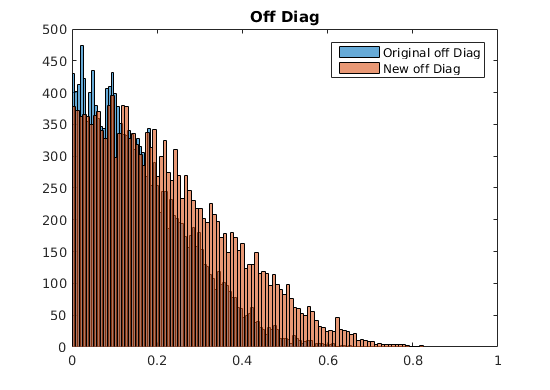
\includegraphics[scale=0.5]{images/Histogram_actual_algo_off_diag}
  \caption{Algo1 Off Diagonal Matrix Comparison}
  \label{fig:1}
\end{figure}

The average relative error in Algo1 case is : 1.163337

The Algo2 gives the following Histogram :
\begin{figure}[H]
  \centering
  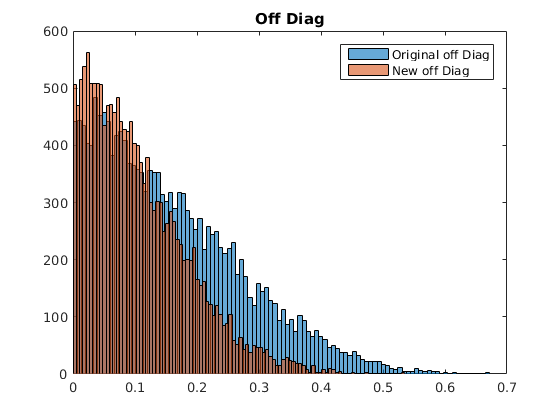
\includegraphics[scale=0.5]{images/Histogram_our_algo_off_diag}
  \caption{Algo2 Off Diagonal Element Histogram}
  \label{fig:2}
\end{figure}
The average relative error in Algo2 case is : 0.147862

\subsection*{A2.2}
\begin{figure}[H]
  \centering
  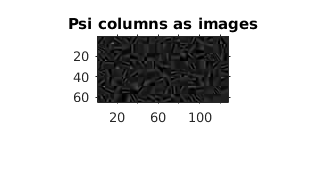
\includegraphics[scale=0.5]{images/Psi_columns_ksvd}
  \caption \\The columns of the matrix $\psi$ rearranged as an image.
  \label{fig:3}
\end{figure}

\subsection*{A2.3}
The plots for Q2c part are as follows:
For Algo1:
\begin{figure}[H]
  \centering
  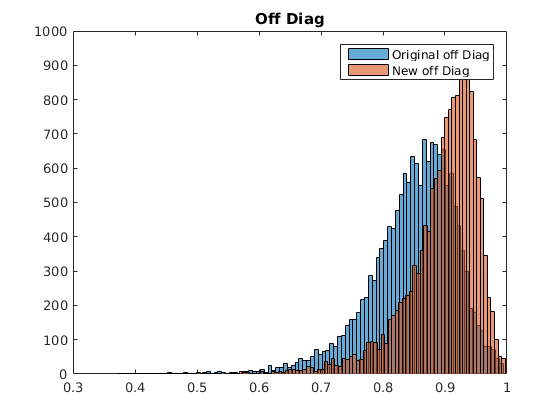
\includegraphics[scale=0.5]{images/q2c_actual_algo}
  \caption{Algo1 plot Hist comparison}
  \label{fig:4}
\end{figure}
The relative error in this case : 1.421040
For Algo2
\begin{figure}[H]
  \centering
  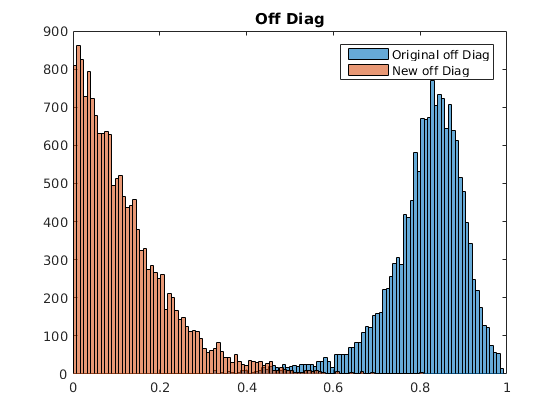
\includegraphics[scale=0.5]{images/q2c_lam_inv}
  \caption{Algo2 plot Hist Comparison}
  \label{fig:5}
\end{figure}
The relative error in this case: 0.161012

\subsection*{A2.4}
The plots for Q2d part are as follows:
For Algo1:
\begin{figure}[H]
  \centering
  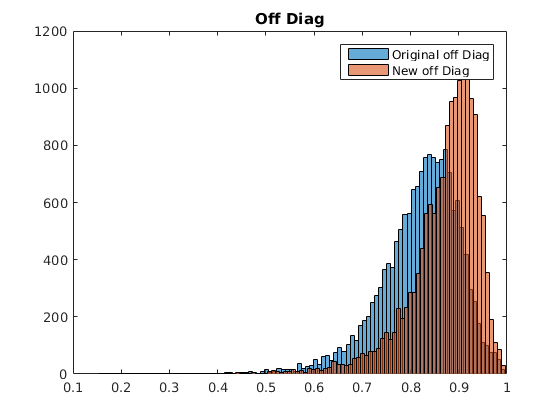
\includegraphics[scale=0.5]{images/q2d_actual_algo}
  \caption{Algo1 plot Hist comparison}
  \label{fig:6}
\end{figure}
The relative error in this case : 1.395116

For Algo2
\begin{figure}[H]
  \centering
  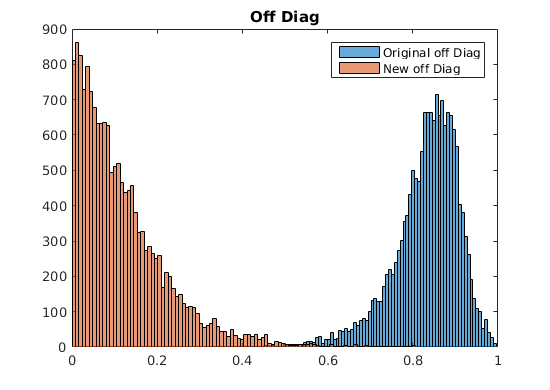
\includegraphics[scale=0.5]{images/q2d_lam_inv}
  \caption{Algo2 plot Hist Comparison}
  \label{fig:7}
\end{figure}
The relative error in this case is 0.377541

\subsection*{A2.E}

The algorithm we have implemented generates a CS matrix with arbitrary real values.
There are multiple problems in the realisation of such a CS matrix

\begin{itemize}
    \item{It is difficult to assign different magnitude of weights to each pixel.
          The accuracy of the hardware will limit the real values to a few quantized 
          levels and hence we will have to use a matrix which performs worse but
          which can be created by the hardware.

        In Hitomi camera, the CS matrix contained only 0s and 1s hence the 
          hardware was a simple cardboard sheet with each pixel having a
          hole(representating 1s) or no hole(representing 0s).
          In our case, we will have to make holes with varying diameters to
          assign different weight to each pixel. These diameters can be created only
          to a certain degree of accuracy and hence we will have to reduce our
          matrix to that accuracy. The error in these diameters will also be higher
          than for a simple CS matrix with 1s and 0s.}


    \item{The CS matrix we have created will require some way to capture negative
    wieghted pixels also. This will require creating a separate hardware matrix
    for positive  and negative values and capturing two compressed measurements
    and subtracting them (The subtraction can be done either before measurement,
    which doubles the amount of hardware used, or can be done after measurement
    in software, which doubles the number of measurements hence reduces
    compression of the setup).}
\end{itemize}


\subsection*{Observations}
We note that this algo is not giving us better results, in almost all cases it is giving us worse relative probability error ($\ge 1$)
 which is an absurd result. Our algorithm on the other hand is giving much better relative error($~0.15$)
\end{document}